%!TeX program = xelatex
%Do not change
\documentclass[12pt, oneside]{article}
\usepackage{amssymb,amsmath}
\usepackage[margin=1in]{geometry}
\usepackage{textpos}
\usepackage{float}
\usepackage{booktabs}
%\usepackage{color}
\usepackage{graphicx}
\usepackage[inter-unit-product =\cdot]{siunitx}
\let\DeclareUSUnit\DeclareSIUnit
\let\US\SI
\DeclareUSUnit\inch{in}
\DeclareUSUnit\foot{ft}
\DeclareUSUnit\mile{mi}
\DeclareUSUnit\foot{ft}
\DeclareUSUnit\slug{slug}
\DeclareUSUnit\pound{lb}
\DeclareUSUnit\psi{psi}
\DeclareUSUnit\Msi{Msi}
\DeclareUSUnit\ksi{ksi}

%\usepackage{tikz}
%\usetikzlibrary{positioning}
%\usepackage{tikz-3dplot}
%\usepackage{pgfopts}
%\usepackage{wasysym}
%\usepackage{stanli}

% You may add the packages you need here
\begin{document}

%TODO change numbers in problems
\begin{textblock*}{4cm}(-1.7cm,-2.3cm)
\noindent {\scriptsize AE333 Fall 2021}
\end{textblock*}

%Do not modify other than putting your name where stated
\begin{textblock*}{8cm}(12.5cm,-1cm)
\noindent {Name: }
\end{textblock*}
%Do not modify other than typing your acknowledgement where stated
\begin{textblock*}{13.5cm}(-1.7cm,-1.8cm)
%\noindent \textit{\footnotesize Acknowledgement: Your acknowledgement for collaboration and other sources goes here. }
\end{textblock*}

\vspace{1cm}

%Do not modify other than typing the homework number after #
\begin{center}
\textbf{\Large Homework 4 Solutions}

\textbf{Due 8 October 2021}
\end{center}

\begin{enumerate}
	\item %p5-1
		Determine the internal torque at each section and sketch the shear stress on a volume element at $A$, $B$, $C$, and $D$.
		\begin{figure}[H]
			\centering
			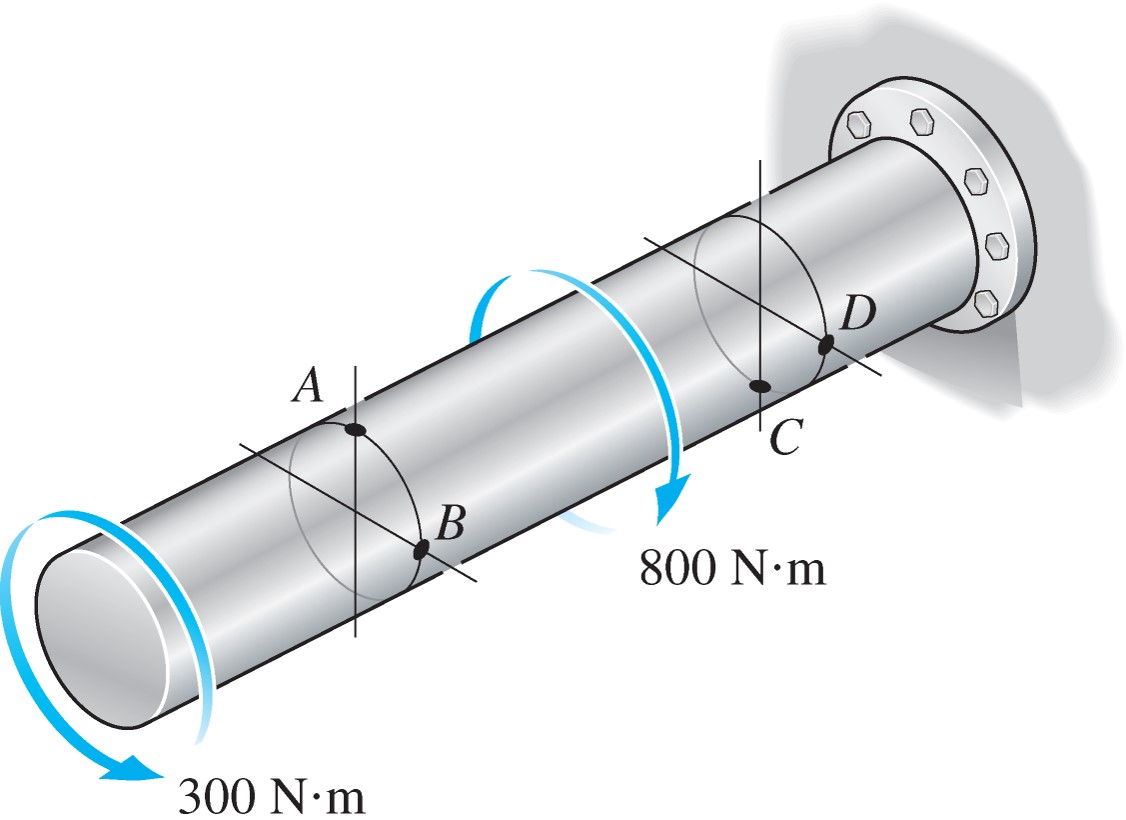
\includegraphics[width=0.6\linewidth]{p5-1}
		\end{figure}
		\textbf{Solution:}
		\begin{itemize}
			\item Looking at the sections shown, we find $T_{AB} = \SI{300}{N.m}$ and $T_{BC} = \SI{-500}{N.m}$
			\begin{figure}[H]
				\centering
				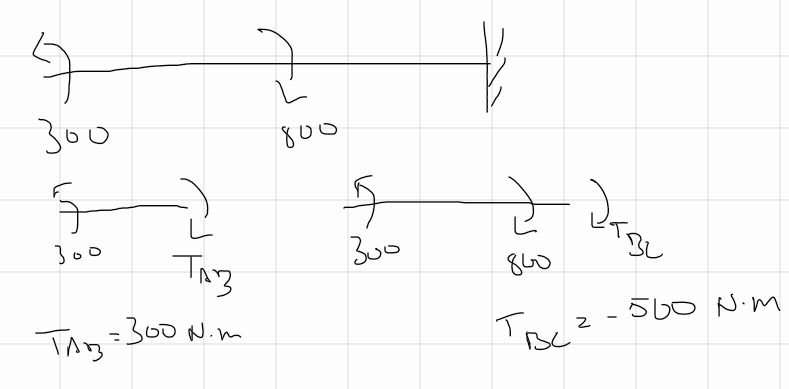
\includegraphics[width=0.6\linewidth]{4-1a}
			\end{figure}
		\item and we can visualize the shear stress on the volume elements as shown
			\begin{figure}[H]
				\centering
				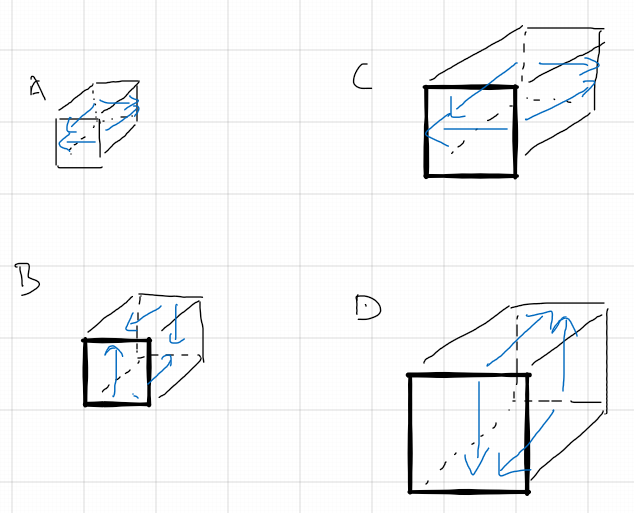
\includegraphics[width=0.6\linewidth]{4-1b}
			\end{figure}
		\end{itemize}
	
	\item %5-28
		The drive shaft $AB$ is to be designed as a thin-walled tube.
		The engine delivers 150 hp while the shaft turns 1000 rpm.
		Find the minimum thickness of the shaft's wall for an outer diameter of $\US{2.5}{in}$ if the allowable shear stress is $\tau_{allow}=\US{6.0}{ksi}$.
		\begin{figure}[H]
			\centering
			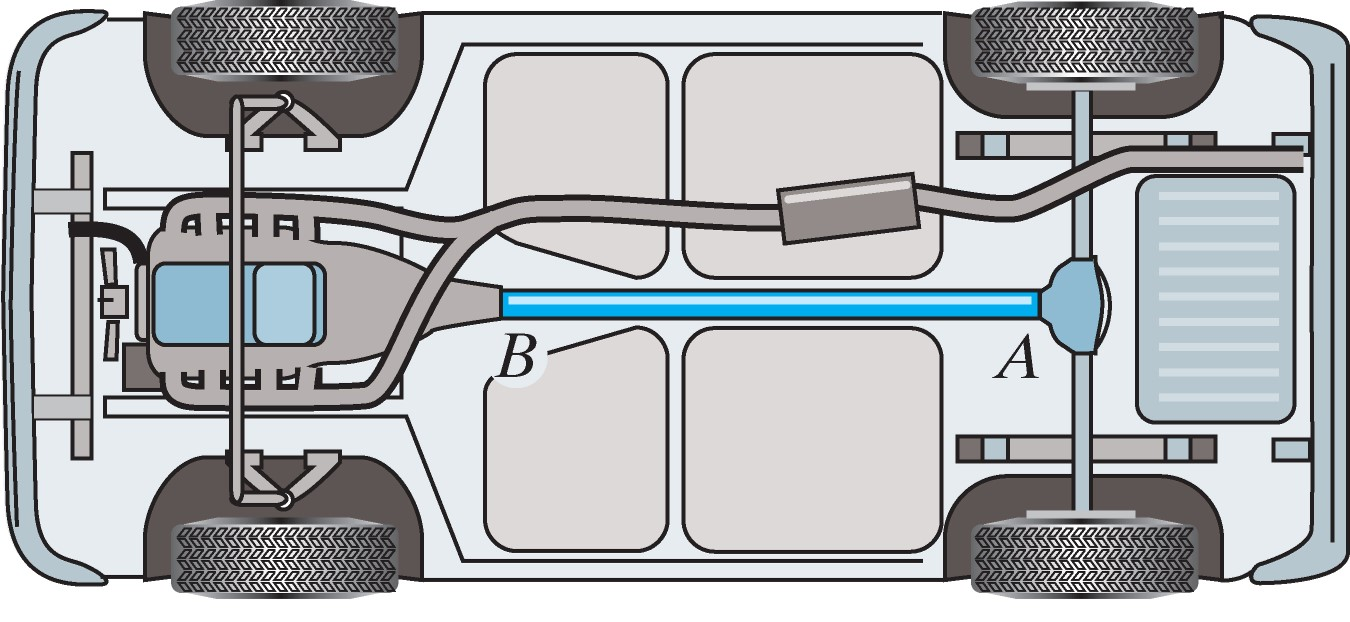
\includegraphics[width=0.6\linewidth]{5-28}
		\end{figure}
		\textbf{Solutions:}
		\begin{itemize}
			\item We can relate power to torque using $P = 2\pi f T$, solving for $T$ we find
				\begin{equation*}
					T = \frac{P}{2\pi f} = \frac{ 150 \text{ hp } }{ 2 \pi 1000 \text{ rpm } } \frac{ 550 \text{ ft lb / s } }{ \text { hp } } \frac{ 60 \text{ sec} }{ \text{ min } } = \US{788}{ft.lb} = \US{9554}{in.lb}
				\end{equation*}
			\item Now we can relate the stress and torque to find the tube thickness, $\tau = \frac{Tc}{J}$, substituting for $J$ we can solve
				\begin{align*}
					\tau &= \frac{Tc}{\pi/2 (c^4 - c_i^4)}\\
					c^4 - c_i^4 &= \frac{2 T c}{\tau \pi}\\
					c_i &= \left( c^4 - \frac{2 T c}{\tau \pi} \right)^{1/4}
				\end{align*}
      \item and we find $c_i = \US{1.04}{in}$ which gives a wall thickness of $\US{0.2}{in} \approx \frac{7}{32}\text{ in}$
		\end{itemize}
    \textbf{Solution Update:} In my original solution, I accidentally lost a 2, the old numbers (with a diameter of 2) gave an impossible result (which means that no inside diameter would work).
    I have updated the problem with a new diameter and corrected my solution.

	\item %5-64
		The soil mixer shown is connected to an A-36 steel tubular shaft with an inside diameter of $\US{1.5}{in}$ and an outside diameter of $\US{3.0}{in}$.
		Determine the angle of twist at $A$ relative to $B$ and the absolute maximum shear stress for the torque shown.
		\begin{figure}[H]
			\centering
			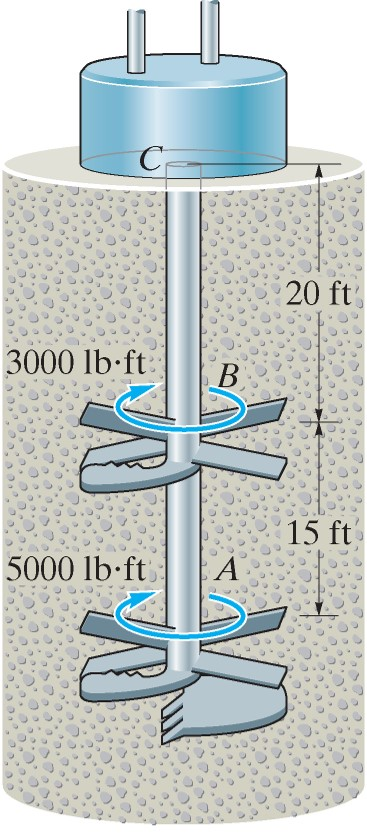
\includegraphics[width=0.2\linewidth]{5-64}
		\end{figure}
		\textbf{Solutions:}
		\begin{itemize}
			\item We start with a simple free body diagram and find that $T_{AB} = \US{5000}{ft.lb}$ and $T_{BC} = \US{8000}{ft.lb}$
			\item The angle of twist between $A$ and $B$ can be found with $\phi = \frac{TL}{JG}$ which for A-36 Steel is $\phi = \frac{\US{60000}{in.lb}\US{180}{in}}{\US{7.455}{in^4}\US{11.0}{Msi}} = 0.132 \text{ rad } = 7.55^\circ$
			\item The shear stress can be found with $\tau = \frac{Tc}{J}$, to find the maximum we use $T_{BC}$ and we find $\tau = \frac{\US{96000}{in.lb}\US{1.5}{in}}{\pi/2(1.5^4-.75^4)} = \US{19.3}{ksi}$
		\end{itemize}

	\item %5-69
		The A-36 Steel bolt shown is tightened such that there is a reactive torque on the shank.
		The reactive torque is expressed as $t = \SI[number-math-rm = \mathnormal, parse-numbers = false]{kx^2 }{N.m/m}$ $k$ has units, but what they are depends on the length unit for $x$.
		If a torque of $T=\SI{45 }{N.m}$ is applied to the bold head find the value of the constant $k$ and the amount of twist in the shank.
		Assume the shank has a radius of $\SI{5 }{mm}$
		\begin{figure}[H]
			\centering
			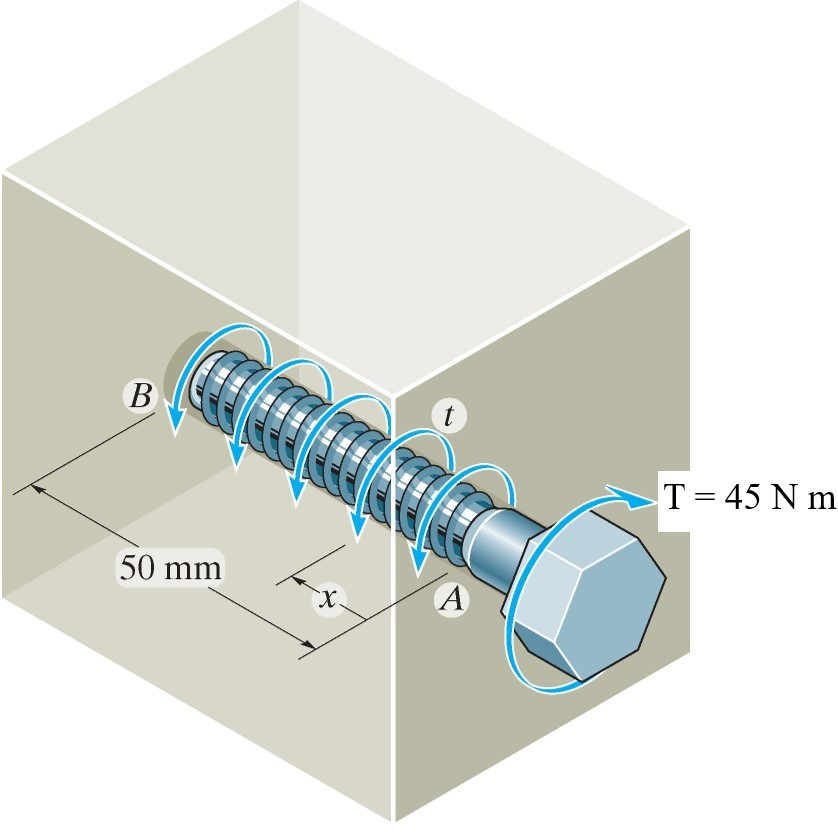
\includegraphics[width=0.6\linewidth]{5-69}
		\end{figure}
		\textbf{Solution:}
		\begin{itemize}
			\item We can see that the reactive torque in the shank must be equal to the applied torque, as there are no other reactions or applied torques
      \item The total torque exerted by this resistance will be the integral of $t$ over the length of the shaft $T_t = \int_0^{50} kx^2 dx = \frac{1}{3}k (50)^3$, which gives $k = \SI{1.08}{N/mm^2}$
		\end{itemize}
    \textbf{Solution Update:} I forgot to calculate the angle of twist in the shank. See below. (I also forgot to include units for $k$, but that has been corrected above)
		\begin{itemize}
			\item We start by sectioning the bolt as shown
				\begin{figure}[H]
					\centering
					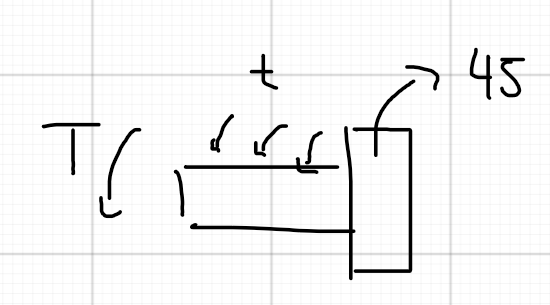
\includegraphics[width=0.6\linewidth]{4-4}
				\end{figure}
			\item To find the internal torque, we need to consider the sum of moments about the $x$ axis (i.e. the sum of torques). To find the total torque exerted by the torsional resistance, $t$, we integrate from $0$ to $x$.
				\begin{equation*}
					\sum T = -T - \int_0^x kx^2 dx + 45 = 0
				\end{equation*}
			\item And we find that $T = 45 - \frac{1}{3}kx^3$, we can now find the total change in angle by integrating the formula for $d\phi$ over the length of the bolt
				\begin{equation*}
					\phi = \int_0^L \frac{T}{JG}dx = \frac{1}{JG}\left( 45L - \frac{1}{12}kL^4 \right)
				\end{equation*}
			\item and we find $\phi = 0.0229 \text{ rad } = 1.31^\circ$
			\item NOTE: make sure units are consistent when performing the calculation, in my case I needed to input $G$ as MPa (for N per square mm) and convert $T$ from N m to N mm.
		\end{itemize}

	\item %5-86
		The aluminum alloy tube (2014-T6, outside) is bonded to an A-36 steel rod (inside) as shown.
		If a torque of $\SI{7 }{kN.m}$ is applied find the maximum shear stress in each material and plot the shear stress as a function of radial position.
		\begin{figure}[H]
			\centering
			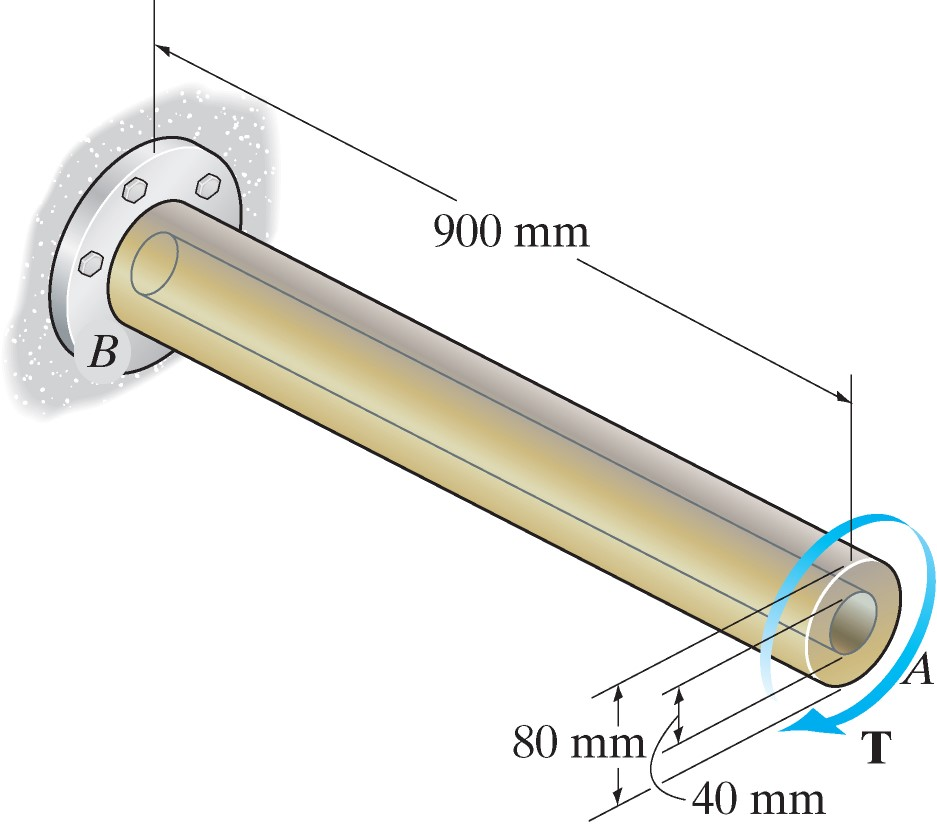
\includegraphics[width=0.6\linewidth]{5-86}
		\end{figure}
		\textbf{Solution:}
		\begin{itemize}
			\item This is a statically indeterminate problem, similar to an example we did in lecture. While we do not know how much of the applied torque is born by the rod and the tube, we do know that the total torque must be equal to the applied torque and that the angle of twist needs to be equal in both.
				\begin{equation*}
					\phi_{al} = \phi_{st} = \left( \frac{TL}{JG} \right)_{al} = \left( \frac{TL}{JG} \right)_{st}
				\end{equation*}
			\item The length is identical in both so that can be canceled, substituting for $J$ and $G$ in both and solving for $T_{st}$ we find
				\begin{equation*}
					T_{st} = \left( \frac{J_{st}G_{st}}{J_{al}G_{al}} \right) T_{al} = 0.185 T_{al}
				\end{equation*}
			\item We know that $T_{st} + T_{al} = \SI{7}{kN.m}$, substituting we can solve for $T_{al} = \SI{5.91}{kN.m}$ and $T_{st} = \SI{1.09}{kN.m}$
			\item We can now substitute known torques into $\tau = \frac{Tc}{J}$ to find the maximum shear stress $\tau_{st} = \SI{87.0}{MPa}$ and $\tau_{al} = \SI{62.7}{MPa}$
				\begin{figure}[H]
					\centering
					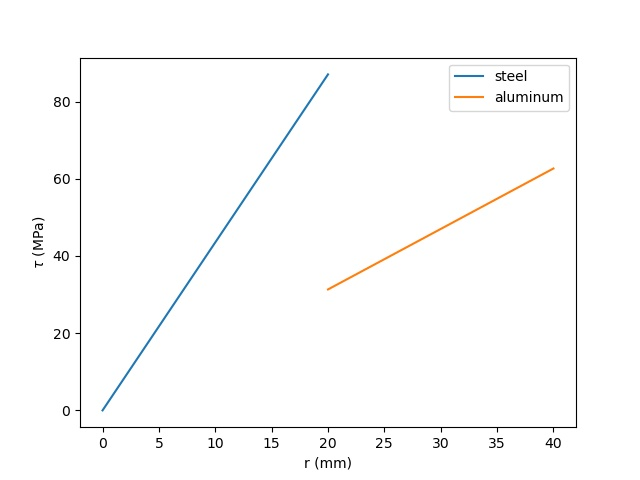
\includegraphics[width=0.6\linewidth]{4-5}
				\end{figure}
		\end{itemize}

	\item %5-109
		For an arbitrary maximum shear stress, compare the torque carrying capacity between two cross-sectional shapes: the circular tube shown (inside) and the rounded rectangular tube (outside) shown.
		For both cases the wall thickness is $\US{0.1}{in}$
		\begin{figure}[H]
			\centering
			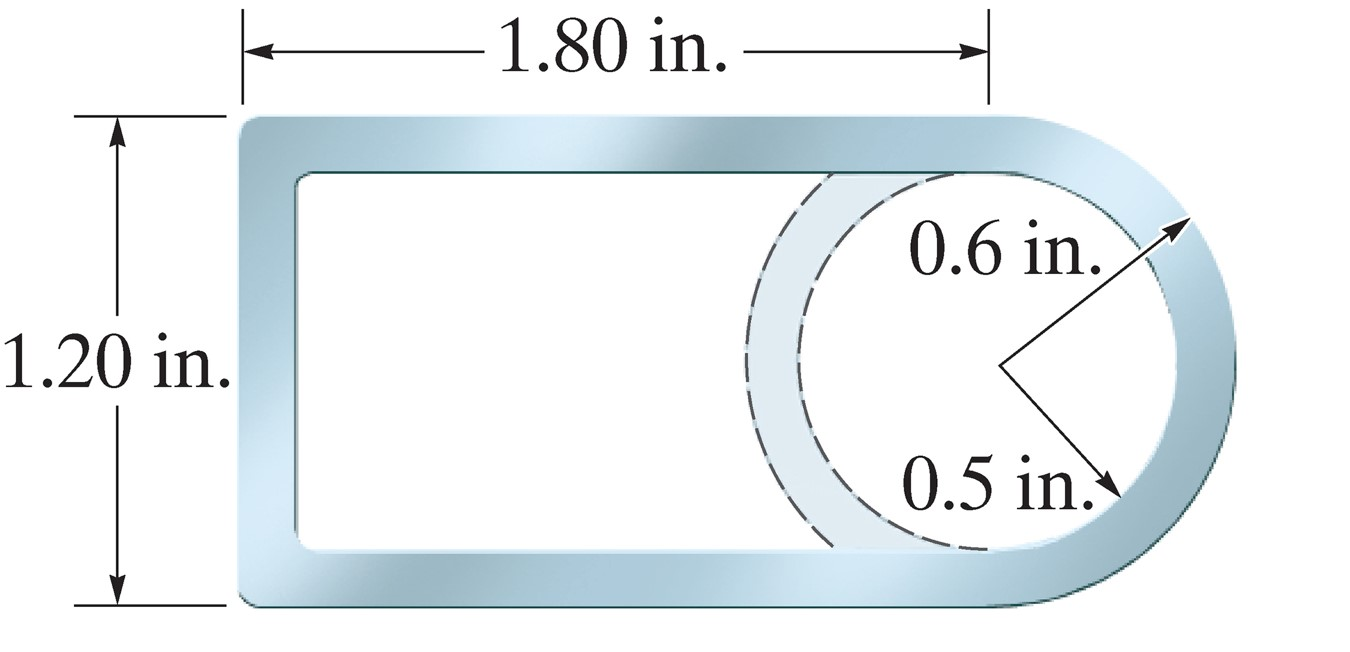
\includegraphics[width=0.6\linewidth]{5-109}
		\end{figure}
		\textbf{Solution:}
		\begin{itemize}
			\item To more directly compare, we'll start by rearranging terms, $\tau = \frac{Tc}{J}$ becomes $T = \left( \frac{J}{c} \right) \tau$
			\item For the non axisymmetric shape, we use shear flow, $T = 2q A_m = (2 t A_m) \tau$
			\item The mean area is calculated as the area inside the midline of the tube, which means $A_m = 1.1(1.75) + \pi/2 (.55^2)$
			\item Substituting known values we find $T_{round} = 0.176 \tau$ and $T_{rect} = 0.480 \tau$, this means the oddly shaped tube can hold a torque 2.7 times higher than the round tube while keeping the same shear stress
		\end{itemize}

\end{enumerate}
\end{document}
